In this chapter the theoretical concepts used throughout the report will be presented. Knowledge of several related, but distinct scientific fields is necessary to understand the following chapters. These are projective geometry, image processing, and image analysis.
% TODO mention radial distortion somewhere
\section{Projective Geometry}
Everyone has a basic understanding of what projective geometry is, and how it works.
We experience it at every wake moment, without thinking about it. 
Based on where one is standing and when looking at a shape, the shape can look very different. % TODO ändra
Projective geometry describes these kinds of phenomena.
In this section some basic concepts in projective geometry is presented, and how images are formed in cameras.

At first glance it seems that very little is preserved by a projective transformation, or "changing perspective" in informal term.
Neither shape, lengths, angles, distances, or ratios of distances are preserved.
The most general property in a scene that is preserved by a projective transformation is straightness. \cite[1]{hartley-zisserman}

In euclidean geometry, a point in two-dimensional space is typically represented by cartesian coordinates, a pair of numbers, which represent the distance to the origin in each dimension. % TODO rephrase
In projective geometry homogeneous coordinates are used instead.
To convert the cartesian coordinate pair $(x,y)$ to homogeneous coordinates, a one is appended to the cartesian coordinates, resulting in the point $(x,y,1)$. 
An interesting property about homogeneous coordinates is that they ignore scale, meaning that $(x,y,1)$ and $(kx,ky,k)$ represents the same point for any nonzero value $k$.
To convert back to cartesian coordinates, divide by $k$ and remove the $1$.\cite[2]{hartley-zisserman} % Rephrase this part

\subsection{Camera Model}\label{camera-model}
Cameras, create a 2D representation of a 3D world.
The camera model used in this thesis is called the projective camera model.
It is based on a pinhole camera model, where all rays of light pass through a single point called the camera centre, $C$. Before reaching $C$, each ray will pierce the image plane, where the image is projected.
It's location is determined by $f$, the focal length of the camera.

\begin{figure}[h]
\begin{center}
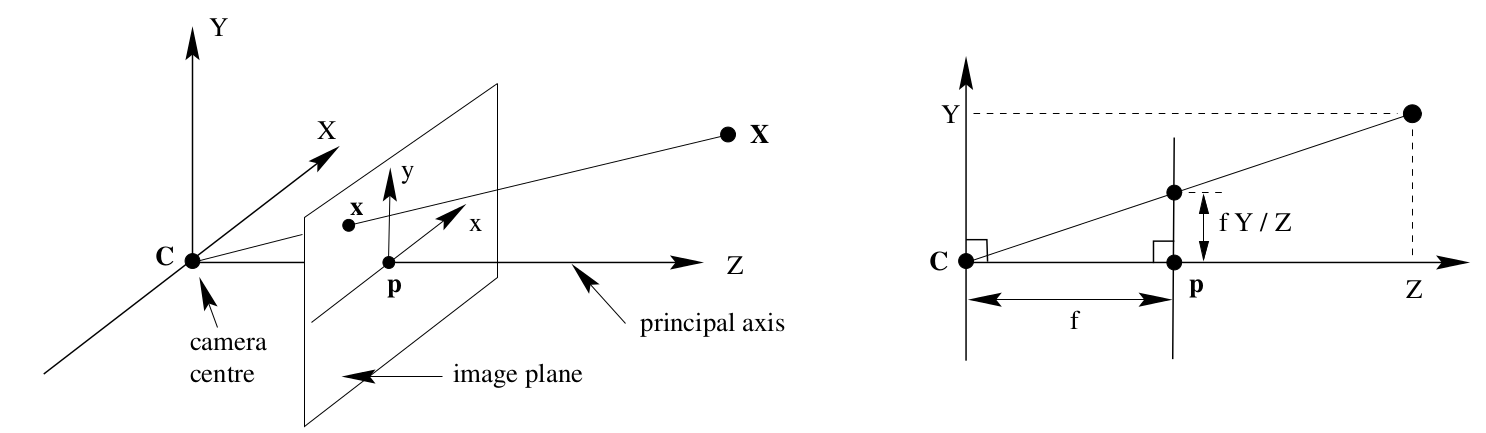
\includegraphics[width=0.6\textwidth]{figures/central_projection_camera.png}
\end{center}
\caption{The central projection camera model. The world and image coordinate systems are aligned. The image plane centred on the $Z$ axis, length $f$ in front of the origin.}
\label{fig:central_projection_camera} % TODO hur referera? zisserman-hartley s.154
\end{figure}

Using the central projection model, as shown in figure \ref{fig:central_projection_camera}, a 3D point can be mapped to a 2D image point, as follows: $(X,Y,Z)^T\mapsto(fX/Z,fY/Z)^T$.
The central projection model makes some rather limiting assumptions, which, which we will now generalise. % TODO is the central projection what is think it is or synonym to the projective camera model???
First, the origin of the image coordinate system is normally not in the centre.
In that case an offset to the principal point, $(p_{x}, p_{y})$, is added, which represents the coordinates of the centre of the image.
Furthermore, the mapping above assumes that the camera is not rotated, and located in the origin of the world coordinate system. Taking this into account, the following equation can be formed:
$$
\begin{pmatrix}	\tilde{u}\\\tilde{v}\\\tilde{w}\end{pmatrix} = 
\begin{pmatrix}
	f & 0 & p_{x} & 0\\
	0 & f & p_{y} & 0\\
	0 & 0 & 1 & 0
\end{pmatrix}
\begin{pmatrix}
	r_{11} & r_{12} & r_{13} & t_{1}\\
	r_{21} & r_{22} & r_{23} & t_{2}\\
	r_{31} & r_{32} & r_{33} & t_{3}
\end{pmatrix}
\begin{pmatrix}	X\\Y\\Z\\1\end{pmatrix}
$$

where $(\tilde{x},\tilde{y},\tilde{z})^T$ are the homogeneous coordinates of the pixel in the image of the world coordinates $(X,Y,Z)$.
As explained earlier, the cartesian coordinates are obtained by dividing by $\tilde{w}$:
$$
u = \frac{\tilde{u}}{\tilde{w}},~~v = \frac{\tilde{v}}{\tilde{w}}
$$
The above is the projective camera model that will be used in this thesis. 
It can be generalised further to take things like pixel skew and non-square pixels into account, but those are rare cases and are therefore left out.

The left of the two matrices above is called the calibration matrix, or intrinsic matrix, $K$.
It contains the intrinsic parameters of the camera.
The intrinsic parameters depend only on the camera, and is always the same for the a given camera, if there is no change in zoom.
The right matrix is called the extrinsic matrix, and contains the extrinsic parameters of the camera.
The extrinsic parameters are not tied to the camera's properties, but instead depend on where in the world the camera is located, and where it points.
The above can also be written in the more concise form $x = K[R|t]X$.

When multiplied together, the intrinsic and extrinsic matrices form a $3\times4$-matrix with 11 degrees of freedom, called the camera matrix, or the projection matrix, $P$:
$$\begin{pmatrix} \tilde{u} \\ \tilde{v} \\ \tilde{w} \end{pmatrix} = \lambda
\begin{pmatrix} p_{11} & p_{12} & p_{13} & p_{14} \\
 				p_{21} & p_{22} & p_{23} & p_{24} \\
				p_{31} & p_{32} & p_{33} & p_{34} \end{pmatrix}
\begin{pmatrix}X \\Y \\Z \\1\end{pmatrix}$$
It can be determined up to an arbitrary scale factor, $\lambda$.
Because $\lambda$ is arbitrary, we simplify to:
$$\begin{pmatrix} \tilde{u} \\ \tilde{v} \\ \tilde{w} \end{pmatrix} =
\begin{pmatrix} p_{11} & p_{12} & p_{13} & p_{14} \\
 				p_{21} & p_{22} & p_{23} & p_{24} \\
				p_{31} & p_{32} & p_{33} & 1 \end{pmatrix}
\begin{pmatrix}X \\Y \\Z \\1\end{pmatrix}$$
where the scaling of the elements of $P$ is implicit for convenience. \cite[153-165]{hartley-zisserman}


\subsection{Planar Homographies}\label{planar-homographies}

\begin{figure}[h]
\begin{center}
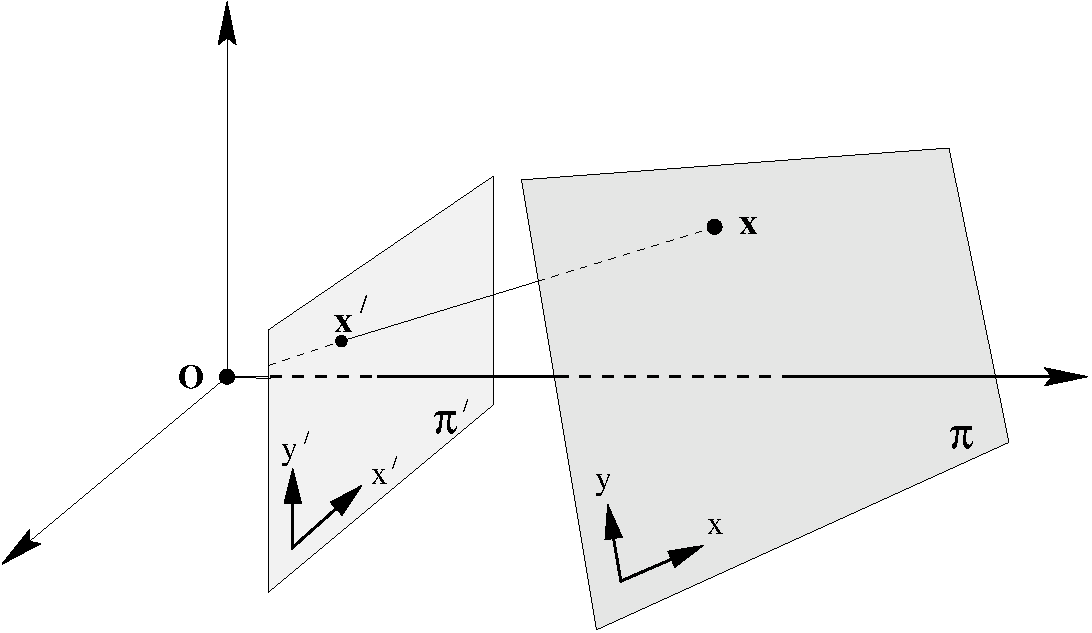
\includegraphics[width=0.6\textwidth]{figures/planar_homography.pdf}
\end{center}
\caption{A point on a plane in the world is projected to the image plane. A planar homography can be used to map points between the two planes} % TODO hur referera? Tagen från hartley-zisserman s. 34
\label{fig:planar_homography}
\end{figure}

Assume that a projective camera is viewing a planar scene, and that we would like to map points on the plane to points on the image plane. 
If the world coordinate system is defined to have its origin in the plane, with the $Z$ axis being perpendicular to it, the projective camera model can be simplified. 
Because $Z=0$ for all coordinates in the plane, the $Z$ coordinate can be removed from the world coordinate vector, along with the third column of the camera matrix, which is cancelled out when $Z=0$. 
This scenario, which is depicted in figure \ref{fig:planar_homography}, yields the following system:
$$\begin{pmatrix} \tilde{u} \\ \tilde{v} \\ \tilde{w} \end{pmatrix} =
\begin{pmatrix} h_{11} & h_{12} & h_{13}  \\
 				h_{21} & h_{22} & h_{23}  \\
				h_{31} & h_{32} & 1\end{pmatrix}
\begin{pmatrix}X \\Y \\ 1\end{pmatrix}$$
This transformation is called a planar homography. 
The above system is also denoted $x=HX$.

$H$ has 8 degrees of freedom, which means that it can be determined with 8 constraints. Each point correspondence adds 2 constraints on $H$, since each point has 2 degrees of freedom.
Hence, a minimum of 4 point correspondences are required to determine $H$.
One method for to determine $H$ from a set of point correspondences is called the Direct Linear Transformation algorithm.
DLT is a simple technique which involves forming constraints based on similarity relations (i.e. the point correspondences), and then solving a linear equation system.
\cite{homography-estimation}

\subsection{Camera Calibration}
This section will describe how to determine the camera matrix $P$, and its components.
This problem is known as camera calibration, or camera resectioning.
It is a very similar problem to the one described in \ref{planar-homographies}, and can be solved in the same manner.
The only difference is that the matrix has an extra column. The number of unknowns is now eleven instead of eight, which means that five and a half point correspondences (meaning five points and one $x$ or $y$ correspondence) are needed instead of four.

The calibration matrix only $K$ only has to be determined once for a given camera.
One approach is to determine it once with good accuracy, and then reuse it even when the extrinsic parameters change.
It is then necessary factorise the camera matrix, to extract $K$, which can be done by RQ-decomposition\cite{qr-decomposition}.

Vanishing points % TODO write

Intrinsic, extrinsic, checkerboard offline calibration, and "online" with vanishing lines TODO! % TODO Vanishing points. Finding pose with known K Mension Zhangs method somehow
\section{Image Processing}
Image processing concerns low-level processing of digital images. 
The input and output of image processing algorithms are images. 
Examples include noise reduction, contrast enhancement, and colour correction. 
The output can however also be some characteristic of the image, such as its average intensity.\cite[p. 1-2]{pitas}\cite[p. 1-2]{gonzalez-woods}

What is interesting to write about here? Filters, Canny % TODO what to write here?

\section{Image Analysis}
Image analysis concerns medium-level processing of digital images. The input is typically an image, and the output a symbolic representation of features in the image. The typical task is image segmentation, i.e. the task of dividing an image into regions and objects. The output could for example represent the contours of an object in the image. \cite[p. 1-2]{pitas}\cite[p. 1-2]{gonzalez-woods}
The field of computer vision can be said to be the next step in the hierarchy. 
The input there is input is typically a low-level symbolic representation of a feature and the output is a high-level symbolic representation. 
The task is for example to understand something about a group of features, to ultimately emulate human vision. \cite[p. 1-3]{pitas}\cite[p. 1-3]{gonzalez-woods}

What is interesting to write about here? Hough lines?

Merge with previous section?
 % TODO what to write here?





















